% ============================================================================
% Supplementary figures for main.tex.  \input this file into si_v0.tex after
% the Supplementary Notes, or paste its contents there.  The figure numbering
% (S1, ...) assumes no other supplementary figures precede it.
% ============================================================================

\renewcommand{\thefigure}{S\arabic{figure}}
\setcounter{figure}{0}

\begin{figure}[htbp]
\centering
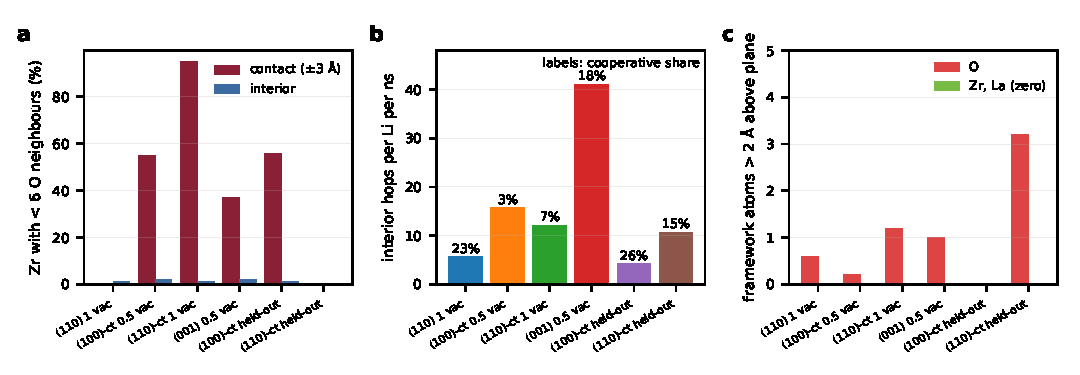
\includegraphics[width=\linewidth]{figs/fig_chemistry.pdf}
\caption{\textbf{Supplementary Figure S1. Interface chemistry at 800~K after
about 3~ns of production.} Means over five replicas for the six interfaces of
Fig.~5. \textbf{a}, Fraction of Zr with fewer than six O neighbours within
2.6~\AA, for Zr within $\pm3$~\AA\ of the interface plane (contact) and for Zr
in the electrolyte interior. The contact value is a property of the as-built
termination (0--96\%) and does not change between 1 and 3~ns; the interior
value is 0--2\% at every temperature. \textbf{b}, Rate of interior lithium hops,
defined as displacements above 2~\AA\ within 2~ps, per lithium per nanosecond;
labels give the share of hops in which a second lithium within 4~\AA\ hops in
the same 2~ps window. \textbf{c}, Framework atoms found more than 2~\AA\ above
the interface plane at the end of the run: 0--3 oxygen per cell and no Zr or La
in any cell. Values are transcribed from
\texttt{data/chemistry\_report\_3ns.md} and plotted by
\texttt{figs/make\_fig\_chemistry.py}.}
\label{fig:chemistry}
\end{figure}
